\lhead{\emph{Securing the Data}}
\chapter{Securing the Data}
The system is designed with one overarching goal. That is to securely capture the remote data and preserve it for later use. For this we have designed a message format that is secure during both collection and transmission. The message data and the event data are carried in the message payload. \autoref{fig:messageDatagram} 
Collecting and storing the data have different security requirements and we treat each with a separate security mechanism. 
During the lifetime of a message, \autoref{fig:messageLifetimeOverviewDiagram} it is created on the node and stored, and later transmitted. While the message is in the stored state, message security properties are confidentiality, integrity, and availability. We refer to this stored state as Message Security. When the system is ready to send, the tasks required to support authentication (both sender integrity and recipient integrity), confidentiality data integrity, and non-repudiation are managed. We refer to this step as Transmission Security.
\begin{figure}
\centering
\includegraphics[scale=.75]{Figures/"message datagram"}
\caption{message datagram}
\label{fig:messageDatagram}
\end{figure}

\begin{figure}
\centering
\includegraphics{Figures/"message lifetime overview diagram"}
\caption{message lifetime overview diagram}
\label{fig:messageLifetimeOverviewDiagram}
\end{figure}

\section{Transmission}
Securing the transmission is divided into two phases. The first phase provides authentication. The outcome of the first phase is the production of a session key. The second phase is the secure transmission of the data confidentially. 
We make use for TLS / SSL for the transmission. TLS / SSL a standarized protocol which will be familar to most readers as it is most often used in securing HTTP. (Browsers reference secured resources with the https protocol identifier.) HTTPS in the browser is, again, most often used to authenticate a server to a browser. This type one way authentication can be augmented with client side authentication. Authentication of both the client and the server is known as mutual authentication.  

\subsection{Certificate Mutual Authentication}
\subsubsection{Phase 1}
In phase one we use x.509 certificates as a means of authenticating the origin of the data.
The certificates required are the ones installed at system provisioning ( $A{_{cert}}$ and $B{_{cert}}$ ). 
The server and the node can trust the certificates to be correct and authentic. The trustworthiness is based on two factors. 
\begin{itemize}
\item The certificates were installed out-of-band of the data and 
\item each server and node has a certificate for the other. 
\end{itemize}
Given that we trust our certificates and that the server and node have each other’s respectively, we can mutual authentication. 
Mutual authentication means that not only does the node know the identity of the server but also the server is confident of the nodes identity. 
Below is a list of steps for mutual authentication diagrammed in \autoref{fig:mutualAuthenticationMessages}:

\begin{enumerate}
\item The node initiates a transmission with a certificate request to the server. 
\item The server responds by sending its certificate. \\ $A{_{cert}}$ \par
\item The server responds with a certificate request for the node and a plaintext message. $m$
\item The node calculates a cyphertext message $m$ encrypted with the nodes private key to produce cyphertext. \\
$c=E{_B{_{priv}}}$
\item The node sends its own certificate $B{_{cert}}$  to the server concatenated with the cyphertext.  \\$B{_{cert}} + c$
\item The server uses the node’s public key, $B{_{pub}}$ , to decrypt the cyphertext and produce its own copy of message $m'$\\$m'=D{_B{_{pub}}}(c)$
\item The server compares $m′$ with the message $m$ that it had sent previously. If $m'$ is equal to $m$ the session moves on to RSA key agreement. \\ $if (m == m')$
\item The key agreement negotiation results in a session key. $k{_session}$ 
\end{enumerate}
 
\begin{figure}
    \centering
    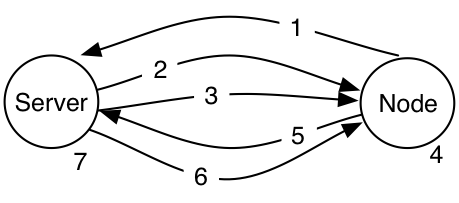
\includegraphics[scale=1, angle=0]{Figures/mutualAuthenticationMessages}
    \caption[Mutual Authentication Messages]{Mutual Authentication Messages}
    \label{fig:mutualAuthenticationMessages}
\end{figure}

The outcome of this first phase is the production of a session key. Using certificates, a chain of trust is established which is used to provide origin integrity for an asymmetric (public/private) key pair. 
These asymmetric keys contained in the certificates are used to verify the identity of the opposite end of the connection and then, once identity has been confirmed, those keys are used in key agreement to establish a session key. 
\cite{Rescorla:2000tv}, \cite{Viega:2002wt}, \cite{Oppliger:2014wm}

\subsection{Secure Communication}
\subsubsection{Phase 2}
The symmetric session key from phase one is now used as a ‘master session key’ from which each transaction will derive an individual key. The use of session keys provides confidentially during transmission. The master key is used to create session keys which also affords us forward secrecy.  

\subsection{Message Security}
The first step in securiting the messsage is securing the payload. 
At this point, the security properties of confidentiality, integrity, and availability are provided.

\section{Message Lifecycle}
The message is instantiated upon the arrival of an event from the node’s input tendril.  The event is recorded in the message payload and a message authentication code (MAC) is applied. The resulting data and MAC are concatenated to produce a record (rx).  \\
$data + MAC = r{_n}$
 
A corresponding symmetric record key, $k{_n}$ is created and used to encrypt the record. Each key is specific to the message. Each message as one key and each key belongs to a single message. The encryption uses this $k{_n}$.  symmetric key generated by the node.  The encryption yields cyphertext $c{_n}$ .  
Confidentiality is provided by the use of encryption while the message is stored. \\
$E{_k{_n}}(r{_n}) = c{_n}$ 

Once encrypted record $c{_n}$ is saved to storage on the node.  

Message records are created by a triggering event may occur at any time. Due to the assumption that we have intermittent communications, availability requires additional handling. Ensuring availability requires that messages be preserved on the remote until they can be transmitted to the data center server. As we show in the section above, the messages are encrypted and stored at the time of instantiation.  When the connection to the data center server becomes available, the messages are transferred. 
% replaced with vector pdf named messageLifetimeOverviewDiagram
%\begin{figure}
%    \centering
%    \includegraphics[scale=.9, angle=0]{Figures/messageLifecycle}
%    \caption[Message Lifecycle]{Message Lifecycle}
%    \label{fig:messageLifecycle}
%\end{figure}
